\chapter{Geometria (2º Bimestre)}

\section{Circunferência, Ângulos, Polígonos}

\subsection*{Circunferência}

As seen in the 5ª série do Ensino Fundamental de Matemática e suas tecnologias,
una circunferência of center $O$ and radius $R$ is the set of points that are
at distance $R$ from $O$.

\begin{center}
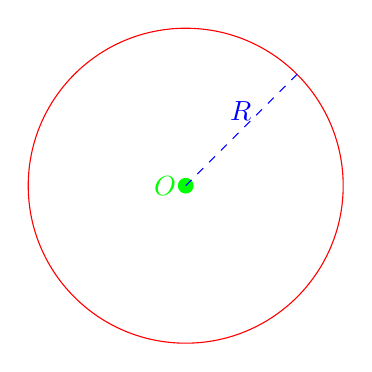
\begin{tikzpicture}
  \draw[red](0,0) circle(2);
  \path[fill=green][green] node[left]{$O$} circle(.1);
  \draw[dashed,blue](0,0) -- (.7,.7)node[above]{$R$} --
  (1.414213562373095,1.414213562373095);
\end{tikzpicture}
\end{center}

Un diámetro es un segmento que une dos puntos en circunferencia y que pasa
por el centro. Si $R$ es la longitud de un radio, los diámetros median
$2R$.

\begin{center}
 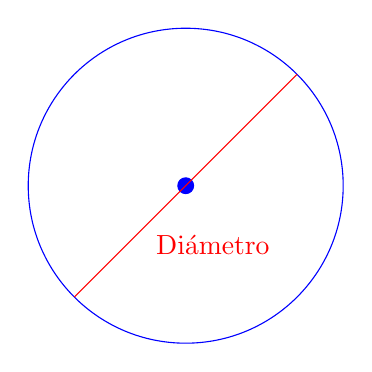
\begin{tikzpicture}
   \draw[color=blue] (0,0) circle(.1)[fill=blue];
   \draw[color=blue] (0,0)  circle(2) (2,0);
   \draw[color=red]
   (-1.414213562373095,-1.414213562373095) --
   (0,0) -- (-0.5,-0.5)node[below right]{Diámetro} --
   (1.414213562373095,1.414213562373095);
 \end{tikzpicture}
\end{center}

De manera más general, un segmento que une dos puntos en circunferencia se
llama un cuerda.

\begin{center}
 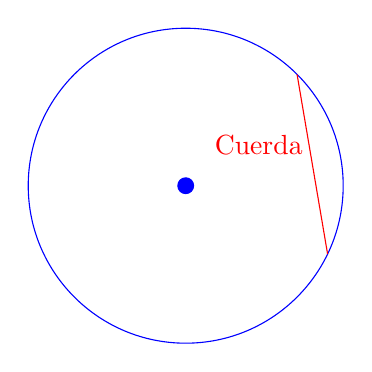
\begin{tikzpicture}
   \draw[color=blue] (0,0) circle(.1)[fill=blue];
   \draw[color=blue] (0,0)  circle(2) (2,0);
   \draw[color=red]
   (1.801937735804838,-0.86776747823511) --
   (1.608075649088966,0.27322304206898)node[above left]{Cuerda} --
   (1.414213562373095,1.414213562373095);
 \end{tikzpicture}
\end{center}

Una cuerda divide la circunferencia en dos partes llamadas arcos.

\begin{center}
 \begin{tikzpicture}
   \draw[color=blue] (0,0) circle(.1)[fill=blue];
   \draw[color=blue]
   (1.801937735804838,-0.86776747823511) --
   (1.414213562373095,1.414213562373095);

   \draw[color=red] (1.414213562373095,1.414213562373095)
   arc(45:0:2) node[above right]{Arco}
   arc(0:-25.71428571428571:2);

   \draw[color=orange] (1.414213562373095,1.414213562373095)
   arc(45:200:2) node[below left]{Arco}
   arc(200:334.2857142857143:2);

 \end{tikzpicture}
\end{center}

\subsection*{Ângulos}

Un ángulo es la parte del plano entre dos semirrectas con el mismo punto de
origen $O$. Un grado (sexagesimal)
es la medida de un ángulo igual a $\frac{1}{360}$ de una circunferencia
de centro $O$.
Si los semirrectas no son coincidentes o alineadas, determinan dos ángulos, uno
convexo (el de menor medida) y otro cóncavo (el de mayor medida).

\begin{center}
\begin{tabular}{| c | c  | c |}
\hline
Tipo & Amplitud & \\
\hline
Ángulo nulo & $A = 0°$ & 
\begin{tikzpicture}
   \draw (0,0) -- (1,0);
 \end{tikzpicture} \\
\hline
Ángulo agudo & $0° < A < 90°$ &
 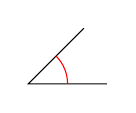
\begin{tikzpicture}
   \draw (1,0) -- (0,0) -- (0.707,0.707);
   \draw (.5,0) arc (0:45:.5)[color=red];
 \end{tikzpicture} \\
\hline
Ángulo recto & $A = 90°$ &
 \begin{tikzpicture}
   \draw (1,0) -- (0,0) -- (0,1);
   \draw (.2,0) -- (.2,.2) -- (0,.2)[color=red];
 \end{tikzpicture} \\
\hline
Ángulo obtuso & $90° < A < 180°$ &
 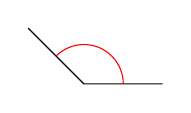
\begin{tikzpicture}
   \draw (1,0) -- (0,0) -- (-0.707,0.707);
   \draw (.5,0) arc (0:135:.5)[color=red];
 \end{tikzpicture} \\
\hline
Ángulo llano & $A = 180°$ & 
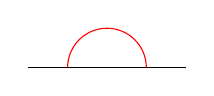
\begin{tikzpicture}
   \draw (1,0) -- (0,0) -- (-1,0);
   \draw (.5,0) arc (0:180:.5)[color=red];
 \end{tikzpicture}\\
\hline
Ángulo oblicuo & $A \neq 0°, 90°, 180°, 270°, 360°$ &\\
\hline
Ángulo completo o perigonal & $A = 360°$&
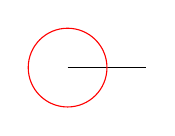
\begin{tikzpicture}
   \draw (0,0) -- (1,0);
   \draw (.5,0) arc (0:360:.5)[color=red];
 \end{tikzpicture} \\
\hline
\end{tabular}
\end{center}

Dos ángulos son complementarios si sus medidas suman 90°:

\begin{center}
 \begin{tikzpicture}
   \draw (0,0) -- (2,0);
   \draw (0,0) -- (1.7320,1);
   \draw (0,0) -- (0,2);
   \draw (0,.2) -- (.2,.2) -- (.2,0);
   \draw (.5,0) arc (0:30:.5)[color=red] node(A){};
   \draw (A) arc (30:90:.5)[color=blue];
 \end{tikzpicture}

\end{center}

Dos ángulos son suplementarios si sus medidas suman 180°:

\begin{center}
 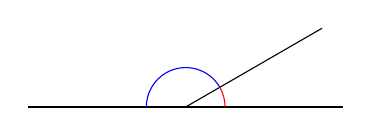
\begin{tikzpicture}
   \draw (0,0) -- (2,0);
   \draw (0,0) -- (1.7320,1);
   \draw (0,0) -- (-2,0);
   \draw (.5,0) arc (0:30:.5)[color=red] node(A){};
   \draw (A) arc (30:180:.5)[color=blue];
 \end{tikzpicture}
\end{center}

En la figura siguiente, los ángulos rojos son dichos opuestos por el vértice.
Son suplementarios del ángulo azul y entonces iguales:

\begin{center}
 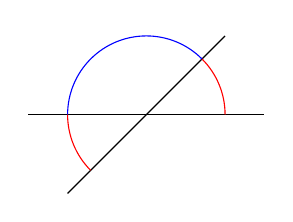
\begin{tikzpicture}
   \draw (-1.5,0) -- (1.5,0);
   \draw (-1,-1) -- (1,1);
   \draw (1,0) arc (0:45:1)[color=red] node(A){};
   \draw (A) arc (45:180:1)[color=blue];
   \draw (-1,0) arc (180:225:1)[color=red];
 \end{tikzpicture}

\end{center}


Consideramos dos rectas paralelas y una transversal a ellas. En la figura
siguiente, los ángulos de mismos colores son dichos correspondientes y tienen
la misma amplitud:

\begin{center}

 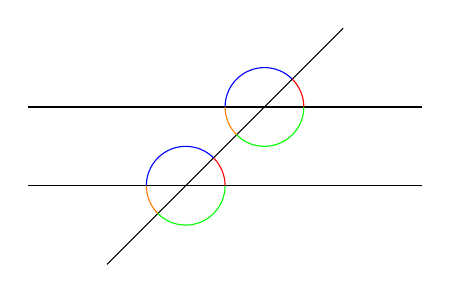
\begin{tikzpicture}
   \draw (0,0) -- (5,0);
   \draw (0,1) -- (5,1);
   \draw (1,-1) -- (4,2);
   \draw (3.5,1) arc (0:45:.5)[color=red] node(A){};
   \draw (A) arc (45:180:.5)[color=blue] node(B){};
   \draw (B) arc (180:225:.5)[color=orange] node(C){};
   \draw (C) arc (225:360:.5)[color=green];

   \draw (2.5,0) arc (0:45:.5)[color=red] node(AA){};
   \draw (AA) arc (45:180:.5)[color=blue] node(BB){};
   \draw (BB) arc (180:225:.5)[color=orange] node(CC){};
   \draw (CC) arc (225:360:.5)[color=green];

 \end{tikzpicture}

\end{center}

En la figura siguiente, los ángulos de mismos colores son dichos
alternos y tienen la misma amplitud:

\begin{center}

 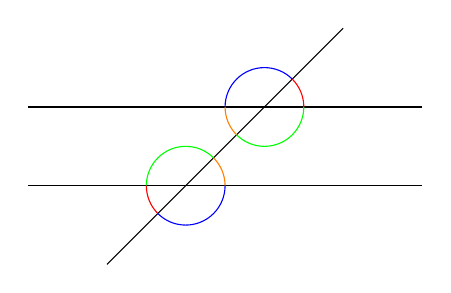
\begin{tikzpicture}
   \draw (0,0) -- (5,0);
   \draw (0,1) -- (5,1);
   \draw (1,-1) -- (4,2);
   \draw (3.5,1) arc (0:45:.5)[color=red] node(A){};
   \draw (A) arc (45:180:.5)[color=blue] node(B){};
   \draw (B) arc (180:225:.5)[color=orange] node(C){};
   \draw (C) arc (225:360:.5)[color=green];

   \draw (2.5,0) arc (0:45:.5)[color=orange] node(AA){};
   \draw (AA) arc (45:180:.5)[color=green] node(BB){};
   \draw (BB) arc (180:225:.5)[color=red] node(CC){};
   \draw (CC) arc (225:360:.5)[color=blue];

 \end{tikzpicture}

\end{center}

\subsection{Exercício 1}

\begin{enumerate}
\item Indique el tipo de los ángulos de medidas siguientes:
  35°, 180°, 45°, 200°, 90°, 350°, 0°, 100°.
\item
  Determine si los ángulos de amplitudes siguientes son complementarios,
suplementarios ningún de los dos:
¿20° y 160°? ¿35° y 65°? ¿28° y 62°? ¿83° y 97°? ¿18° y 172°?
\item Indique el ángulo complementario y suplementario de los ángulos
  siguientes de amplitudes siguientes: 20°, 57°, 88°, 0°, 90°.
\end{enumerate}

\subsection{Exercício 2}

Consideramos dos rectas paralelas y una transversal a ellas.
Indique los ángulos que son correspondiente y alternos con el ángulo rojo.
¿Si la amplitud del ángulo azul es 145°, cuales son las amplitudes de los otros?

\begin{center}

 \begin{tikzpicture}
   \draw (0,0) -- (8,0);
   \draw (0,2) -- (8,2);
   \draw (1,-1) -- (7,3);

   \draw (6.5,2) arc (0:35:1)[color=red] node(A){};
   \draw (A) arc (35:180:1)[color=blue] node(B){};
   \draw (B) arc (180:215:1)[color=green];

   \draw (3.5,0) arc (0:35:1)[color=purple];
   \draw (1.5,0) arc (180:215:1)[color=orange];

 \end{tikzpicture}

\end{center}

\subsection{Polígonos}

In the 3º Bimestre de la
5ª série do Ensino Fundamental de Matemática e suas tecnologias,
we also defined um polígono as a sequence of segmentos
${[A_1,A_2]}, {[A_2, A_3]}, {[A_3, A_4]},\ldots,
{[A_{n-1},A_n]}, {[A_{n},A_1]}$ forming a closed shape. We also saw
simple/complex, convex/concave, regular polygons as well as various names of
polygons according to the number of sides.

\begin{center}
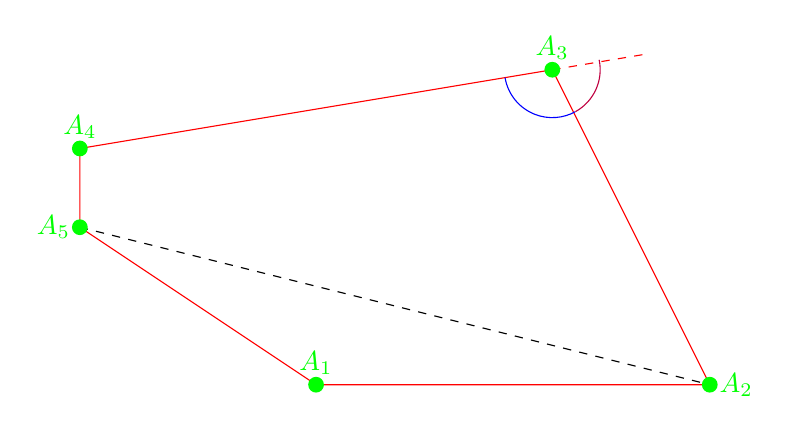
\begin{tikzpicture}
  \draw[red](0,0) -- (5,0) -- (3,4) -- (-3,3) -- (-3,2) -- (0,0);
  \draw[dashed] (-3,2) -- (5,0);
  \draw[dashed,red] (3,4) -- (4.2,4.2);
  \path[fill=green][green] (0,0) node[above]{$A_1$} circle(.1);
  \path[fill=green][green] (5,0) node[right]{$A_2$} circle(.1);
  \path[fill=green][green] (3,4) node[above]{$A_3$} circle(.1);
  \path[fill=green][green] (-3,3) node[above]{$A_4$} circle(.1);
  \path[fill=green][green] (-3,2) node[left]{$A_5$} circle(.1);
  \draw[blue](2.4,3.9) arc (189.4623222080256:299:0.608276253029822) node(A){};
  \draw[purple] (A) arc (-61:12:0.608276253029822);
\end{tikzpicture}
\end{center}

Wikipedia da las definiciones siguientes:

\begin{itemize}
\item Lado: es cada uno de los segmentos que conforman el polígono.
  For example ${[A_1,A_2]}, {[A_2, A_3]}, {[A_3, A_4]},\ldots$
\item Vértice: es el punto de intersección (punto de unión) de dos lados consecutivos. For example $A_1, A_2, A_3, \ldots$
\item Diagonal: es el segmento que une dos vértices no consecutivos.
  For example $[A_2A_5]$ is drawn in dash.
\item Ángulo interior de un polígono simple: es el ángulo formado, internamente al polígono, por dos lados consecutivos.
  For example
  $\widehat{A_2A_3A_4} = \widehat{A_3}$ is drawn in blue.
\item Ángulo exterior de un polígono simple convexo: es el ángulo formado,
  externalmente al polígono,
  por un lado y la prolongación de un lado consecutivo.
  For example the angle drawn in purple, corresponding to $A_3$.
\item Centro de un polígono regular: es el punto equidistante de todos los vértices y lados.
\item Ángulo central de un polígono regular:
  es el formado por dos segmentos de recta que parten del centro a los extremos
  de un lado.
\item Apotema de un polígono regular: es el segmento que une el centro del polígono con el centro de un lado; es perpendicular a dicho lado.
\end{itemize}

\subsection{Exercício 3}

Consideramos un polígono con $n \geq 3$ lados.

\begin{itemize}
\item ¿Cuantos vértices tiene?
\item ¿Cuantos diagonales tiene?
\item ¿Si es regular, cual es la medida de un ángulo central minimal?
  ¿Y la suma de esos ángulos centrales?
\end{itemize}

\subsection{Exercício 4 (sum of the angles of a triangle)}

In the following figure, what is the sum of the red, green and blue angles?
What is the sum of the interior angles (orange, green, cyan) of the triangle?

\begin{center}

 \begin{tikzpicture}
   \draw (0,0) -- (8,0);
   \draw (0,2) -- (8,2);
   \draw (1,-1) -- (7,3);
   \draw (5.2,2.6) -- (7,-1);
   
   \draw (4.5,2) arc (180:215:1)[color=red] node(A) {};
   \draw (A) arc (215:297:1)[color=green] node(B) {};
   \draw (B) arc (297:360:1)[color=blue];
   
   \draw (3.5,0) arc (0:35:1)[color=orange];
   \draw (5.5,0) arc (180:118:1)[color=cyan];

 \end{tikzpicture}

\end{center}

\subsection{Exercício 5}

\begin{itemize}
\item Represente sobre una figura los ángulos interiores y exteriores de
  un triángulo.
\item Deduzca la suma de los ángulos exteriores de un triángulo.
\item Sean $A, B, C$ tres vértices consecutivos de un $n$-gono
  simple convexo ($n \geq 4$).
  Represente sobre una figura los ángulos interiores y exteriores
  $\alpha, \beta, \gamma$
  en $A, B, C$.
\item Si retiramos el punto $B$, exprese la suma de los nuevos
  ángulos exteriores en $A$ y $C$.
\item Deduzca la suma de los ángulos exteriores de un poligóno simple convexo.
\item Exprese la suma de los angúlos interiores del $n-1$-gono ($B$ retirado).
  en función de la suma de los angúlos interiores del $n$-gono.
\item Deduzca la suma de los ángulos interior de un poligóno simple convexo.
\end{itemize}

\section{Simetrias and Construções geométricas}

\subsection*{Tools and Construções geométricas}

In order to do construções geométricas, you can use various tools:

\begin{enumerate}
\item uma régua to draw retas or verify that three points are aligned.
\item uma régua graduada to measure distance or place points on uma reta.
\item a compasso to draw circle or report distances.
\item a esquadro to draw uma reta orthogonal to another one or verify that
  two retas are orthogonal.
\item a transferidor to measure angles or draw angles of a given measure.
\end{enumerate}

Given two points, you can use uma régua to draw the line passing by these two
points. Given one point and uma reta you can use the esquadro to draw the reta
orthogonal passing by the point.

\begin{center}
 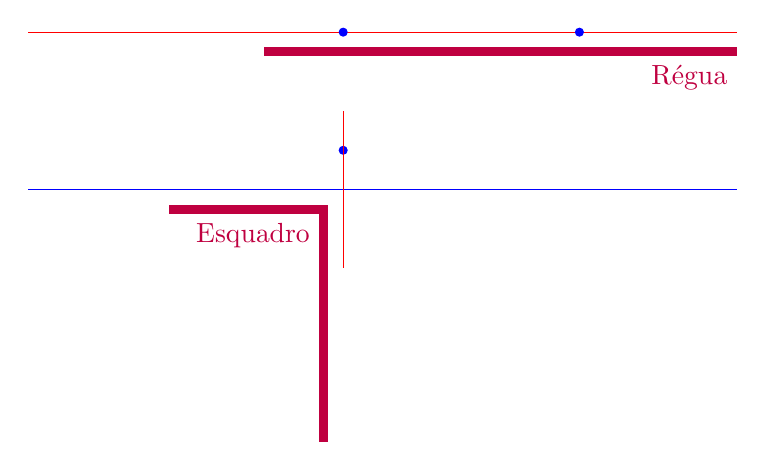
\begin{tikzpicture}
   \draw[color=red] (-4,0) -- (5,0);
   \draw[fill=blue] (0,0) circle(.05)[color=blue];
   \draw[fill=blue] (3,0) circle(.05)[color=blue];

   \begin{scope}[shift={(2,-.2)}]
      \draw[color=purple,fill=purple](0,0) --
      (-3,0) -- (-3,-.1) -- (3,-.1) node[below left]{Régua} --
      (3,0) -- cycle;
    \end{scope}

   
  \begin{scope}[shift={(0,-2)}]
    \draw[color=blue] (-4,0) -- (5,0);
    \draw[fill=blue] (0,.5) circle(.05)[color=blue];
    \draw[color=red] (0,1) -- (0,-1);

    \begin{scope}[shift={(-.2,-.2)}]
      \draw[color=purple,fill=purple](0,0) --
      (-2,0) -- (-2,-.1) -- (-.1,-.1) node[below left]{Esquadro} --
      (-.1,-3) -- (0,-3) -- cycle;
    \end{scope}
    
  \end{scope}
 \end{tikzpicture}
\end{center}

Using the esquadro again, you can also
draw the reta parallel passing by the point:

\begin{center}
 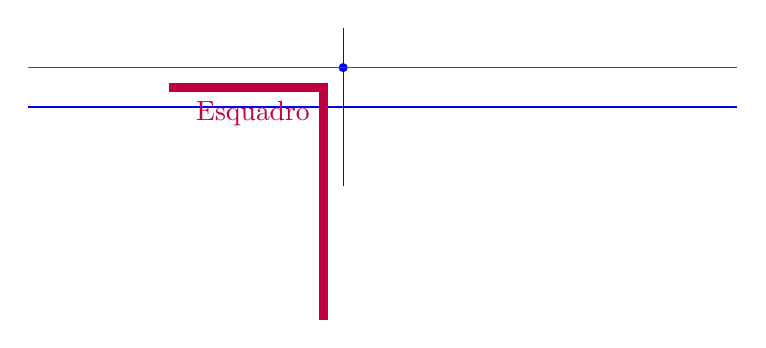
\begin{tikzpicture}
  \begin{scope}[shift={(0,-2)}]
    \draw[color=blue] (-4,0) -- (5,0);
    \draw[fill=blue] (0,.5) circle(.05)[color=blue];
    \draw[color=blue] (0,1) -- (0,-1);
    \draw[color=red] (-4,.5) -- (5,.5);

    \begin{scope}[shift={(-.2,.3)}]
      \draw[color=purple,fill=purple](0,0) --
      (-2,0) -- (-2,-.1) -- (-.1,-.1) node[below left]{Esquadro} --
      (-.1,-3) -- (0,-3) -- cycle;
    \end{scope}
    
  \end{scope}
 \end{tikzpicture}
\end{center}

Given two points, you can use the compasso to
draw two circles centered at these points and large
enough so that they intersect into two points. You can trace the reta passing
by these two points, which is called the mediatrice of the segment made by
the two original points.

\begin{center}
 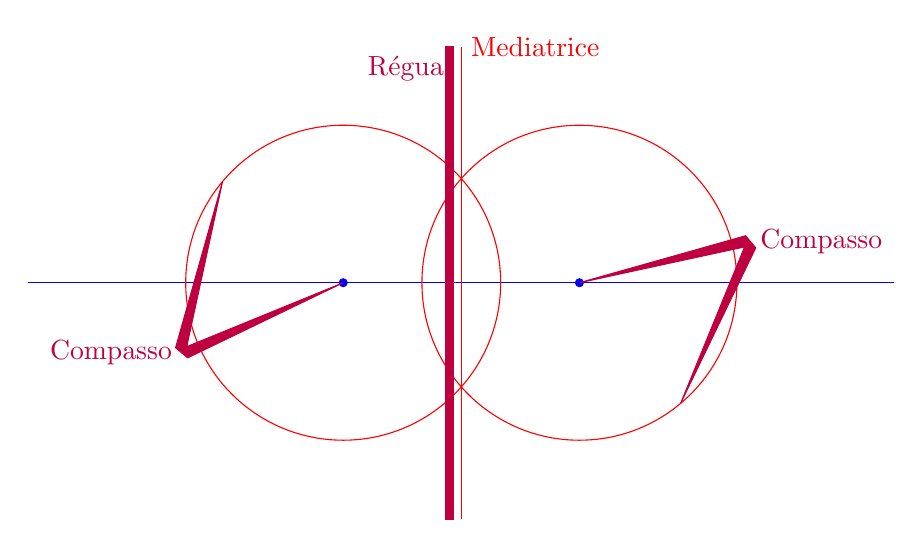
\begin{tikzpicture}
   \draw[color=blue] (-4,0) -- (7,0);
   \draw[fill=blue] (0,0) circle(.05)[color=blue];
   \draw[fill=blue] (3,0) circle(.05)[color=blue];
   \draw[color=red] (0,0) circle(2)[color=red];
   \draw[color=red] (3,0) circle(2)[color=red];

   \draw[color=red] (1.5,-3) -- (1.5,3)  node[right]{Mediatrice};
   \begin{scope}[shift={(1.3,0)},rotate=90]
      \draw[color=purple,fill=purple](0,0) --
      (-3,0) -- (-3,-.1) -- (3,-.1) node[below left]{Régua} --
      (3,0) -- cycle;
    \end{scope}

   
  \begin{scope}[shift={(3,0)},rotate=40]
  \draw[color=purple,fill=purple](0,0) --
  (2,-.9) -- (2,-1) node[right]{Compasso} --
  (2,-1.1) -- (0,-2) -- (1.9,-1) -- cycle;
  \end{scope}

    \begin{scope}[shift={(0,0)},rotate=-130]
  \draw[color=purple,fill=purple](0,0) --
  (2,-.9) -- (2,-1) node[left]{Compasso} --
  (2,-1.1) -- (0,-2) -- (1.9,-1) -- cycle;
  \end{scope}

 \end{tikzpicture}
\end{center}

Given three points $A,B,C$, we can draw the angle $\widehat{ABC}$ using the
régua. Using the compasso, we draw a circle intersecting $[BA)$ and
$[BC)$ into two points $E,F$. We can then construct the mediatrice of the
segment $[EF]$ as above. This reta splits $\widehat{ABC}$ into two half
and is called the bissectrice of $\widehat{ABC}$.

\begin{center}
 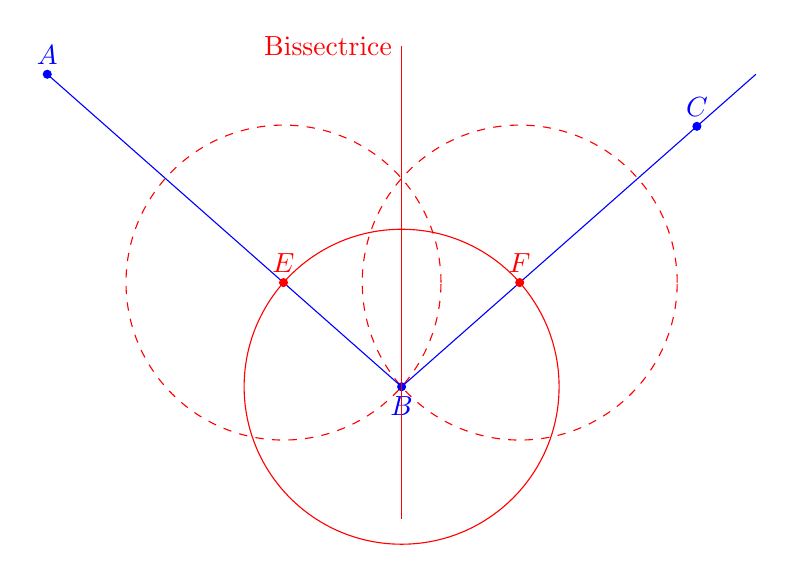
\begin{tikzpicture}
   \draw[color=red,dashed] (0,0) circle(2)[color=red];
   \draw[color=red,dashed] (3,0) circle(2)[color=red];
   \draw[color=red] (1.5,-1.322875655532295) circle(2)[color=red];
   \draw[color=blue]
   (-3,2.64575131106459) --
   (0,0) -- (1.5,-1.322875655532295) -- (3,0) -- (6,2.64575131106459);
   \draw[fill=red] (0,0) circle(.05)[color=red]  node[above]{$E$};
   \draw[fill=blue] (1.5,-1.322875655532295) circle(.05)[color=blue] node[below]{$B$};
   \draw[fill=red] (3,0) circle(.05)[color=red]  node[above]{$F$};
   \draw[color=red] (1.5,-3) -- (1.5,3) node[left]{Bissectrice};

   \draw[fill=blue] (-3,2.64575131106459) circle(.05)[color=blue] node[above]{$A$};
   \draw[fill=blue] (5.25,1.984313483298442) circle(.05)[color=blue] node[above]{$C$};

 \end{tikzpicture}
\end{center}

\subsection*{Exercício 6}

In this exercise, we only use compasso and régua.

\begin{enumerate}
\item Given two points $P,Q$, draw the middle of $[PQ]$.
\item Given uma reta $\mathcal{R}$ and a point $P$
  Draw a circle of center $P$ that is large enough to intersect
  $\mathcal{R}$ into two points $Q,R$. Draw the mediatrice of $[QR]$. What
  can you say about that reta?
\item Given uma reta $\mathcal{R}$ and a point $P$, draw the reta parallel
  to $\mathcal{R}$ passing by $P$.
\end{enumerate}

We now consider a triangle $ABC$.

\begin{enumerate}
\item Draw the mediatrices of $[AB]$, $[BC]$, $[AC]$.
  They intersect at one point $P_1$. Draw the circle of center $P_1$ passing
  by $A$. What do you notice?
\item Deduce $Q_1,Q_2,Q_3$ as the midpoints of $[AB]$, $[BC]$, $[CD]$.
\item Draw the bissectices of the internal angles of $ABC$. They intersect at
  one point $P_2$. Draw the reta passing by $P_2$ perpendicular to $(AB)$ and
  consider its insersection point with $(AB)$.
  Draw the circle of center $P_2$ passing by that intersection point.
  What do you notice?
\item Draw the reta orthogonal to $(BC)$ passing by $A$. This
  is called an altitude of $ABC$. Draw the two other altitudes. They intersect
  at one point $P_3$ called the orthocenter. What do you notice with respect
  to $P_1,P_2$?
\item Deduce $Q_4,Q_5,Q_6$ as the intersections of each altitude
  with the corresponding side as well as $Q_7,Q_8,Q_9$ the midpoints of each
  segment $[AP_3]$, $[BP_3]$, $[CP_3]$.
  As in the first question, draw the circle passing by $Q_1,Q_2,Q_3$.
  What do you notice?
\item Draw the reta passing by $A$ and the middle of $[BC]$. This is called
  a median of $ABC$. Draw the two other medianes. What do you notice?
\end{enumerate}
  
\subsection*{Simetrias}

According to Wikipedia:

\begin{enumerate}
\item Em geometria, o eixo de simetria é uma linha que divide uma figura em
  duas partes simétricas, isto é, como se fossem o objeto e a sua imagem num
  espelho.
\item Um objeto com simetria de rotação é um objeto que tem a mesma aparência
  depois de um determinado montante de rotações.
  O grau de simetria rotacional é quantos graus a forma inicial
  tem que ser girada para se parecer com a mesma de um lado ou em um vértice
  diferente.
\end{enumerate}

\subsection*{Exercício 7}

Describe the symetries in the following geometric figures:

\begin{enumerate}
\item
    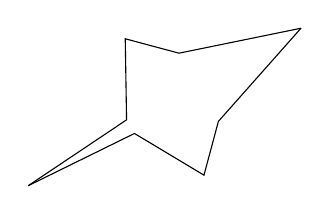
\begin{tikzpicture}
      \begin{scope}[scale=.5,rotate=30]
      \draw(0,0) -- (3,.2) -- (4,2) -- (5, 1) -- (8,0);
      \begin{scope}[yscale=-1.0]
        \draw(0,0) -- (3,.2) -- (4,2) -- (5, 1) -- (8,0);
      \end{scope}
    \end{scope}
    \end{tikzpicture}
  
\item 
    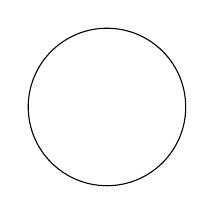
\begin{tikzpicture}
      \draw(0,0) circle(1);
    \end{tikzpicture}

\item 
    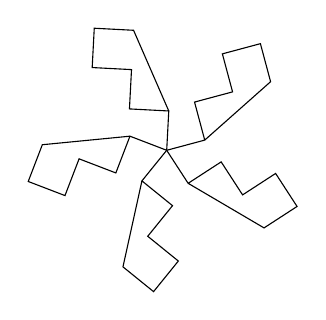
\begin{tikzpicture}
      \begin{scope}[scale=.5,rotate=15]
      \begin{scope}[rotate=0]
        \draw(0,0) -- (1,0) -- (1,1) -- (2,1) -- (2,2) -- (3,2) --
        (3,1) -- (1,0);
      \end{scope}
      \begin{scope}[rotate=72]
        \draw(0,0) -- (1,0) -- (1,1) -- (2,1) -- (2,2) -- (3,2) --
        (3,1) -- (1,0);
      \end{scope}
      \begin{scope}[rotate=144]
        \draw(0,0) -- (1,0) -- (1,1) -- (2,1) -- (2,2) -- (3,2) --
        (3,1) -- (1,0);
      \end{scope}
      \begin{scope}[rotate=216]
        \draw(0,0) -- (1,0) -- (1,1) -- (2,1) -- (2,2) -- (3,2) --
        (3,1) -- (1,0);
      \end{scope}
      \begin{scope}[rotate=288]
        \draw(0,0) -- (1,0) -- (1,1) -- (2,1) -- (2,2) -- (3,2) --
        (3,1) -- (1,0);
      \end{scope}
      \end{scope}
    \end{tikzpicture}
    
\item

    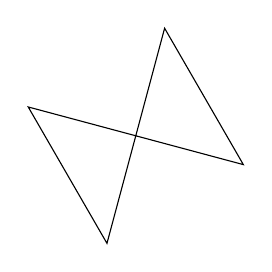
\begin{tikzpicture}
      \begin{scope}[rotate=-60]
      \draw(0,0) -- (2,2) -- (0,2) -- (2, 0) -- cycle;
    \end{scope}
    \end{tikzpicture}


\end{enumerate}

\subsection*{Exercício 8 (polígonos regulares)}

\begin{enumerate}
\item Use your rule to draw uma reta $\mathcal{R}_1$.
  Use your compasso and graduated rule to draw a circle $\mathcal{C}_4$
  of radius $4\text{cm}$ whose center belongs to la reta $\mathcal{R}_1$.
  $\mathcal{R}_1$ and $\mathcal{C}_4$ intersect into two points $A,C$.
\item Use your compasso to draw the mediatriz $\mathcal{R}_2$ of $[AC]$.
\item $\mathcal{R}_1$ and $\mathcal{C}_4$ intersect into two points $B,D$.
  What is the simple polygons
  inscribed in $\mathcal{C}_4$ made by the points $A,B,C,D$?
\item Use your compasso to draw a regular polygon
  of size $4$ inscrito en $\mathcal{C}_4$. ¿Cómo se llama?
\item Draw un triángulo equilátero inscrito en $\mathcal{C}_4$.
\item Use your compasso and graduated rule to draw a circle $\mathcal{C}_3$
  of radius $3\text{cm}$ as well as one of its diameter $\mathcal{D}$.
  With your rule, place $E$ a
  point on $\mathcal{D}$ splitting it into two segments of length $1$ and $5$.
\item Use your compasso to draw the circle
  $\mathcal{C}_1$ of center $E$ and radius $1\text{cm}$.
  Use your esquadro to draw la reta $\mathcal{R}_1$ passing by $E$
  and orthogonal to the diameter $\mathcal{D}$.
\item $\mathcal{R}_1$ intersects $\mathcal{C}_1$ and $\mathcal{C}_3$ at four
  points and thus three segments. Use
  your compasso to draw the circle $\mathcal{C}_{\sqrt{5}-1}$
  with same center as $\mathcal{C}_4$ and radius the
  length of one of the longest segment.
\item $\mathcal{C}_{\sqrt{5}-1}$ intersects $\mathcal{R}_1$ at two points.
  Let $F$ be the closest to $A$.
  Use your esquadro to draw la reta $\mathcal{R}_3$
  passing by $F$ and orthogonal to $\mathcal{R}_1$.
\item $\mathcal{R}_1$ intersects $\mathcal{C}_1$ into two points $G,H$.
  Use your compasso to draw a regular polygon inscrito en $\mathcal{C}_4$
  that has $AG$ and $AH$ as two of its sides. ¿Cómo se llama?
\item
  Let $\beta$ be a central angle of the equilateral triangle previously
  constructed and $\alpha$ be a minimal central angle of the polygon constructed
  in the previous question?
  Use your compasso to construct the bissectrice of the angles
  $\alpha, \beta$. Construct dos polígonos regulares inscritos en
  $\mathcal{C}_4$ de ángulos centrales minimales
  $\frac{\alpha}{2}$ y $\frac{\beta}{2}$. ¿Cómo se llaman?
\item Construct un octógono y hexadecágono ($16$-gono) regulares
  inscritos en $\mathcal{C}_4$.
\item Construct un polígono regular inscrito en $\mathcal{C}_4$ y
  ángulo central minimal $2 \alpha - \beta$. ¿Cómo se llama?
\item For each regular polygon constructed, measure with your transferidor the
  a minimal central angle and an interior angle. Is it expected?
\item What are the simetrias axiales e de rotação of a regular polygon?
\item Did you really need uma régua graduada and a esquadro to draw these
  polygons?
\end{enumerate}

\section{Poliedros}

Quoting Wikipedia:

Um poliedro é um sólido geométrico cuja superfície é composta por um número
finito de faces, cujos vértices são formados por três ou mais arestas em três
dimensões em que cada uma das faces é um polígono. Os seus elementos mais
importantes são as faces, as arestas e os vértices.

\subsection*{Exercício 9}

Exercício 8 provides a way to draw a regular pentagon. By repeating the
pentagon shape, reproduce the following
planification on a paper. Cut and build the corresponding poliedro. Indicate
its number of faces $F$, the number of arestas $A$ e the number vértices $V$.
Verify the teorema de Euler: $V + F = A + 2$.

    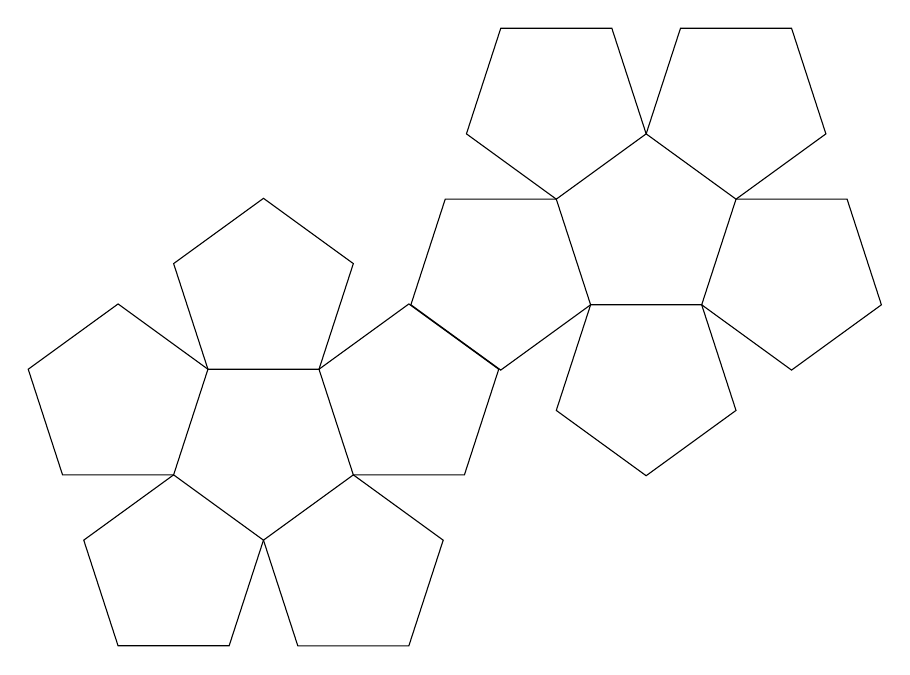
\begin{tikzpicture}
      \begin{scope}[scale=.3]

        \begin{scope}[rotate=18]
      \begin{scope}[rotate=0,shift={(6.472135954999579,0)}]
        \draw (4, 0) -- (1.23606797749979,3.804226065180614) --
        (-3.236067977499789,2.351141009169893) --
        (-3.236067977499789,-2.351141009169892) --
        (1.23606797749979,-3.804226065180614) -- cycle;
      \end{scope}

      \begin{scope}[rotate=72,shift={(6.472135954999579,0)}]
        \draw (4, 0) -- (1.23606797749979,3.804226065180614) --
        (-3.236067977499789,2.351141009169893) --
        (-3.236067977499789,-2.351141009169892) --
        (1.23606797749979,-3.804226065180614) -- cycle;
      \end{scope}

      \begin{scope}[rotate=144,shift={(6.472135954999579,0)}]
        \draw (4, 0) -- (1.23606797749979,3.804226065180614) --
        (-3.236067977499789,2.351141009169893) --
        (-3.236067977499789,-2.351141009169892) --
        (1.23606797749979,-3.804226065180614) -- cycle;
      \end{scope}

      \begin{scope}[rotate=216,shift={(6.472135954999579,0)}]
        \draw (4, 0) -- (1.23606797749979,3.804226065180614) --
        (-3.236067977499789,2.351141009169893) --
        (-3.236067977499789,-2.351141009169892) --
        (1.23606797749979,-3.804226065180614) -- cycle;
      \end{scope}

      \begin{scope}[rotate=288,shift={(6.472135954999579,0)}]
        \draw (4, 0) -- (1.23606797749979,3.804226065180614) --
        (-3.236067977499789,2.351141009169893) --
        (-3.236067977499789,-2.351141009169892) --
        (1.23606797749979,-3.804226065180614) -- cycle;
      \end{scope}
        \end{scope}

        \begin{scope}[shift={(16.2,9.2)},rotate=198]
      \begin{scope}[rotate=0,shift={(6.472135954999579,0)}]
        \draw (4, 0) -- (1.23606797749979,3.804226065180614) --
        (-3.236067977499789,2.351141009169893) --
        (-3.236067977499789,-2.351141009169892) --
        (1.23606797749979,-3.804226065180614) -- cycle;
      \end{scope}

      \begin{scope}[rotate=72,shift={(6.472135954999579,0)}]
        \draw (4, 0) -- (1.23606797749979,3.804226065180614) --
        (-3.236067977499789,2.351141009169893) --
        (-3.236067977499789,-2.351141009169892) --
        (1.23606797749979,-3.804226065180614) -- cycle;
      \end{scope}

      \begin{scope}[rotate=144,shift={(6.472135954999579,0)}]
        \draw (4, 0) -- (1.23606797749979,3.804226065180614) --
        (-3.236067977499789,2.351141009169893) --
        (-3.236067977499789,-2.351141009169892) --
        (1.23606797749979,-3.804226065180614) -- cycle;
      \end{scope}

      \begin{scope}[rotate=216,shift={(6.472135954999579,0)}]
        \draw (4, 0) -- (1.23606797749979,3.804226065180614) --
        (-3.236067977499789,2.351141009169893) --
        (-3.236067977499789,-2.351141009169892) --
        (1.23606797749979,-3.804226065180614) -- cycle;
      \end{scope}

      \begin{scope}[rotate=288,shift={(6.472135954999579,0)}]
        \draw (4, 0) -- (1.23606797749979,3.804226065180614) --
        (-3.236067977499789,2.351141009169893) --
        (-3.236067977499789,-2.351141009169892) --
        (1.23606797749979,-3.804226065180614) -- cycle;
      \end{scope}
        \end{scope}
        
        \end{scope}
    \end{tikzpicture}

\subsection*{Exercício 10}

\begin{enumerate}
\item Draw a planification of the cube.
\item Cut and build a cube. Count its number
  of faces, arestas e vértices. Verify the theorem of Euler.
\item Draw the cube in perspective and draw the center of each faces.
\item What is the poliedro convexo made by joining these centers?
  Count its number
  of faces, arestas e vértices. Verify the theorem of Euler.
\end{enumerate}

\section{Solução dos exercícios}

\subsection*{Exercício 1}

\begin{enumerate}
\item agudo y oblicuo, llano, agudo y oblicuo, oblicuo, recto, oblicuo, nulo,
  obtuso y oblicuo.
\item suplementario, ningún de los dos, complementario, suplementario,
  ningún de los dos
\item
Las medidas de los ángulos complementarios son 70°, 33°, 2°, 90°, 0°.
Las medidas de los ángulos suplementarios son 160°, 123°, 92°, 90°, 180°.
\end{enumerate}

\subsection*{Exercício 2}

El ángulo naranja es alterno con el ángulo rojo, el ángulo ṕurpuro es
correspondiente con el ángulo rojo. Los ángulos rojo y verde son opuestos
por el vértice y entonces iguales. Por la primera pregunta,
es también la medida de los ángulos naranja y ṕurpuro.

\subsection*{Exercício 3}

\begin{itemize}
\item Hay dos vértices para cada lados, y cada vértice apartene a dos lados
  entonces hay $\frac{2n}{2} = n$ vértices. Podemos también decir los
  vértices son exactamente los puntos de salida (o de llegada) de los
  lados, y entonces hay $n$ vértices. Por ejemplo, un triángulo tiene tres
  vértices, un cuadrilatero cuatro vértices etc
\item Para obtener un diagonal, elegimos un punto ($n$ posibilidades) y
  otro que no es conectado con el primer ($n-3$ posibilidades). Para cada
  diagonal hay dos posibilidades para el primer punto elegido y entonces
  hay $\frac{n{(n-3)}}{2}$ diagonales. Por ejemplo, un triángulo no tiene 
  diagonal, un cuadrilatero tiene dos diagonales, un pentágono tiene
  cinco diagonales etc
\item Una vuelta completa es 360°. Para un ángulo central (minimal), sólo
  es $\frac{1}{n}$ de una vuelta completa, es decir $\frac{360}{n}$. La suma
  de esos ángulos centrales es 360°.
\end{itemize}

\subsection*{Exercício 4 (sum of the angles of a triangle)}

These angles form a straight line so their sum is 180°. The red and orange
angles are alternate and thus equal. The blue and cyan angles are
alternate and thus equal. Finally the sum of the angles of the triangle
is 180°.

\subsection*{Exercício 5}

Los ángulos rojos son los ángulos interiores y
los ángulos azules son los ángulos exteriores. La suma de los ángulos interiores
es $x+y+z=180°$.
Además, cada par de ángulo interior/exterior coresponde a
ángulos suplementarios. Entonces la suma de los ángulos exteriores es
${(180° - x)} + {(180° - y)} + {(180° - z)} = 3\times180° - {(x+y+z)} = 360°$.

\begin{center}
 \begin{tikzpicture}
   \draw (0,0) -- (3,0) -- (2,1) -- (0,0);
   \draw[dashed] (3,0) -- (4,-1);
   \draw[dashed] (2,1) -- (4,2);
   \draw[dashed] (0,0) -- (-2,0);

   \draw[color=red](.5,0) arc(0:26:.5) node(A){};
   \draw[color=blue](A) arc(26:180:.5);

   \draw[color=blue](2.5,0) arc(180:316:.5);
   \draw[color=red](2.5,0) arc(180:136:.5);

   \draw[color=blue](2.449397023149583,1.219185573394538) arc(26:-43:.5) node(B){};
   \draw[color=red](B) arc(-43:-152:.5);

 \end{tikzpicture}
\end{center}

Los ángulos rojos son los ángulos interiores y los
ángulos azules son los ángulos exteriores.

\begin{center}
 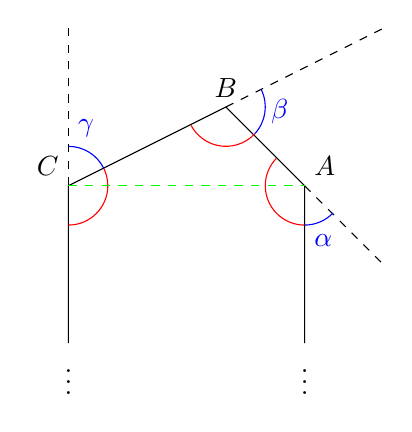
\begin{tikzpicture}
   \draw (0,-2)node[below]{$\vdots$} -- (0,0)node[above left]{$C$} -- (2,1)
   node[above]{$B$} -- (3,0)node[above right]{$A$} --
   (3,-2)node[below]{$\vdots$};
   \draw[dashed] (3,0) -- (4,-1);
   \draw[dashed] (2,1) -- (4,2);
   \draw[dashed] (0,0) -- (0,2);

   \draw[color=red](0,-.5) arc(-90:26:.5) node(A){};
   \draw[color=blue](A) arc(26:90:.5) node[above right]{$\gamma$};

   \draw[color=blue](3,-.5)node[below right]{$\alpha$} arc(270:316:.5);
   \draw[color=red](3,-.5) arc(270:136:.5);

   \draw[color=blue](2.449397023149583,1.219185573394538)
   node[below right]{$\beta$} arc(26:-43:.5) node(B){};
   \draw[color=red](B) arc(-43:-152:.5);

   \draw[dashed,color=green] (0,0) -- (3,0);

 \end{tikzpicture}
\end{center}

Si retiramos el punto $B$, la amplitud del ángulo exterior en $A$ se vuelve
$\alpha + \widehat{CAB}$ y la amplitud del ángulo exterior en $C$ se vuelve
$\gamma + \widehat{BCA}$. Entonces la suma de estes dos ángulos es
$\alpha + \gamma + \widehat{CAB} + \widehat{BCA} =
\alpha + \gamma + {(180° - \widehat{ABC})} = \alpha+\beta+\gamma$.
Por lo tanto, la suma de los ángulos exteriores de un
$n$-gono es la misma que la suma de los angúlos interiores de un $n-1$-gono,
de un $n-2$-gono, $n-3$-gono... y finalmente de un triángulo es decir 360°.

De la misma manera, para obtener la suma de los angúlos interiores en el
$n-1$-gono a partir de la suma del $n$-gono,
restamos el ángulo interior $\widehat{ABC}$,
restamos $\widehat{CAB}$ del ángulo interior en $A$ y
restamos $\widehat{BCA}$ del ángulo interior en $C$. Entonces restamos
$\widehat{ABC}+\widehat{CAB}+\widehat{BCA}=180°$. Al final,
la suma de los ángulos interiores de un triángulo es $180°$, la de un
cuadrado $180+180=360°$, ... y la de un $n$-gono $180\times {(n-2)}$°.

Note que las definiciones y resultados pueden ser generalizados a polígonos
que no son simple o convexo.


\subsection*{Exercício 6}

\begin{enumerate}
\item This is done by drawing the mediatrice of $[PQ]$ and considering its
  intersection with $[PQ]$.
\item We obtain the reta passing by $P$ and orthogonal to $\mathcal{R}$
  (without using the esquadro).
\item We first draw the reta $\mathcal{R'}$ orthogonal to $\mathcal{R}$
  and passing by $P$ as in the previous question. Then again, we draw the
  reta orthogonal to $\mathcal{R'}$ passing by $P$. This is the reta parallel
  to $\mathcal{R}$ passing by $P$.
\end{enumerate}

\begin{enumerate}
\item We get the circle passing by the vertices $A,B,C$ of the triangle,
  called the circle circumscribed.
\item These are the intersections with the sides and their mediatrice.
\item We get the inscribed circle: the largest circle contained in $ABC$.
  It is tangent to each side.
\item $P_3$ is aligned with $P_1,P_2$.
\item This circle also passes by $Q_4,Q_5,Q_6,Q_7,Q_8,Q_9$. It is called
  the nine-point circle or Euler's circle.
\item The three medians intersect at one point (called the centroid).
\end{enumerate}

\subsection*{Exercício 7}

\begin{enumerate}
\item
  Clearly $(AB)$ is an axis of symmetry.
  The shape is a simple polygon.
  The internal angle $\widehat{A}$ is not equal to any
  other internal angle of the polygon, so it must be preserved by a symmetry.
  Hence we don't have any rotational symmetry (of non-zero grau). Similarly the
  internal angle corresponding to vertex $B$ must be preserved by a symmetry.
  Hence there is no other axis of symmetry than $(AB)$.
  
    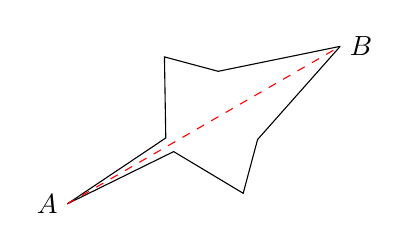
\begin{tikzpicture}
      \begin{scope}[scale=.5,rotate=30]
        \draw(0,0)node[left]{$A$} -- (3,.2) -- (4,2) -- (5, 1) -- (8,0)
        node[right]{$B$};
      \begin{scope}[yscale=-1.0]
        \draw(0,0) -- (3,.2) -- (4,2) -- (5, 1) -- (8,0);
      \end{scope}
      \draw[color=red,dashed](0,0) -- (8,0);
      \end{scope}
    \end{tikzpicture}
  
  \item This is a circle of center $O$. Any reta passing by $O$
    provides an axial symmetry of the circle.
    For any $n \geq 2$, we have a rotational symmetry of center
    $O$ and grau $n$.
    Any symmetry preserving the circle must preserve its center $O$,
    so there is not any more possibility.
    
    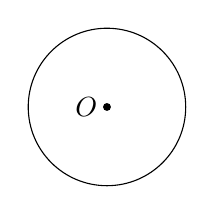
\begin{tikzpicture}
      \fill(0,0) circle(.05);
      \draw(0,0) node[left]{$O$} circle(1);
    \end{tikzpicture}

  \item As in the previous case, a symmetry preserving the shape must preserve
    the center $O$ so it must be either be an axial symmetry
    for a reta passing by $O$ or a rotational symmetry of center
    $O$ and grau $n$. Actually, a symmetry must preserve the small
    red ``branches''  intersecting at the point $O$ so we can only
    have a rotational symmetry of grau $n = 5$ or an axial symmetry
    whose axis includes one of this red branch. One can verify that the former
    provides a rotational symmetry for the whole shape but the latter does not.

  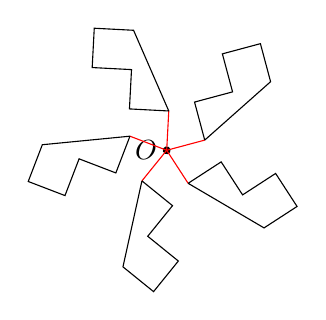
\begin{tikzpicture}
      \begin{scope}[scale=.5,rotate=15]
      \fill(0,0) node[left]{$O$}circle(.1);
      \begin{scope}[rotate=0]
        \draw(0,0) -- (1,0)[red];
        \draw(1,0) -- (1,1) -- (2,1) -- (2,2) -- (3,2) -- (3,1) -- (1,0);
      \end{scope}
      \begin{scope}[rotate=72]
        \draw(0,0) -- (1,0)[red];
        \draw(1,0) -- (1,1) -- (2,1) -- (2,2) -- (3,2) -- (3,1) -- (1,0);
      \end{scope}
      \begin{scope}[rotate=144]
        \draw(0,0) -- (1,0)[red];
        \draw(1,0) -- (1,1) -- (2,1) -- (2,2) -- (3,2) -- (3,1) -- (1,0);
      \end{scope}
      \begin{scope}[rotate=216]
        \draw(0,0) -- (1,0)[red];
        \draw(1,0) -- (1,1) -- (2,1) -- (2,2) -- (3,2) -- (3,1) -- (1,0);
      \end{scope}
      \begin{scope}[rotate=288]
        \draw(0,0) -- (1,0)[red];
        \draw(1,0) -- (1,1) -- (2,1) -- (2,2) -- (3,2) -- (3,1) -- (1,0);
      \end{scope}
      \end{scope}
    \end{tikzpicture}
    
\item This is a complex polygon with two segments intersecting at point
  $O$. So again $O$ must be preserved and actually these two segments
  intersecting at $O$ must either be preserved or be exchanged by the symmetry.
  We finally find a rotational symmetry of center $O$ and grau $2$ and
  two axial symmetries provided by the axis in red and blue.

    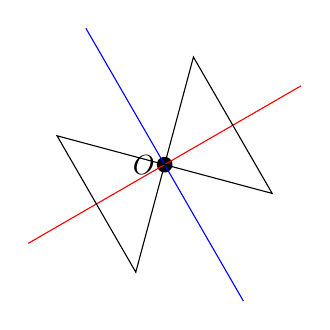
\begin{tikzpicture}
      \begin{scope}[rotate=-60]
      \fill(1,1) node[left]{$O$}circle(.1);
      \draw[red](1,-1) -- (1,3);
      \draw[blue](-1,1) -- (3,1);
      \draw(0,0)  -- (2,2) -- (0,2) -- (2, 0) -- cycle;
    \end{scope}
    \end{tikzpicture}


\end{enumerate}

\subsection*{Exercício 8}

We first get the following schemas. The regular polygon $ABCD$ is a square
(in red)! The regular polygon of size $4$ inscrito en $\mathcal{C}_4$ is
an hexagon (green). Considering one vertix over two, we get the triángulo
equilátero inscrito en $\mathcal{C}_4$ (orange).

\begin{center}
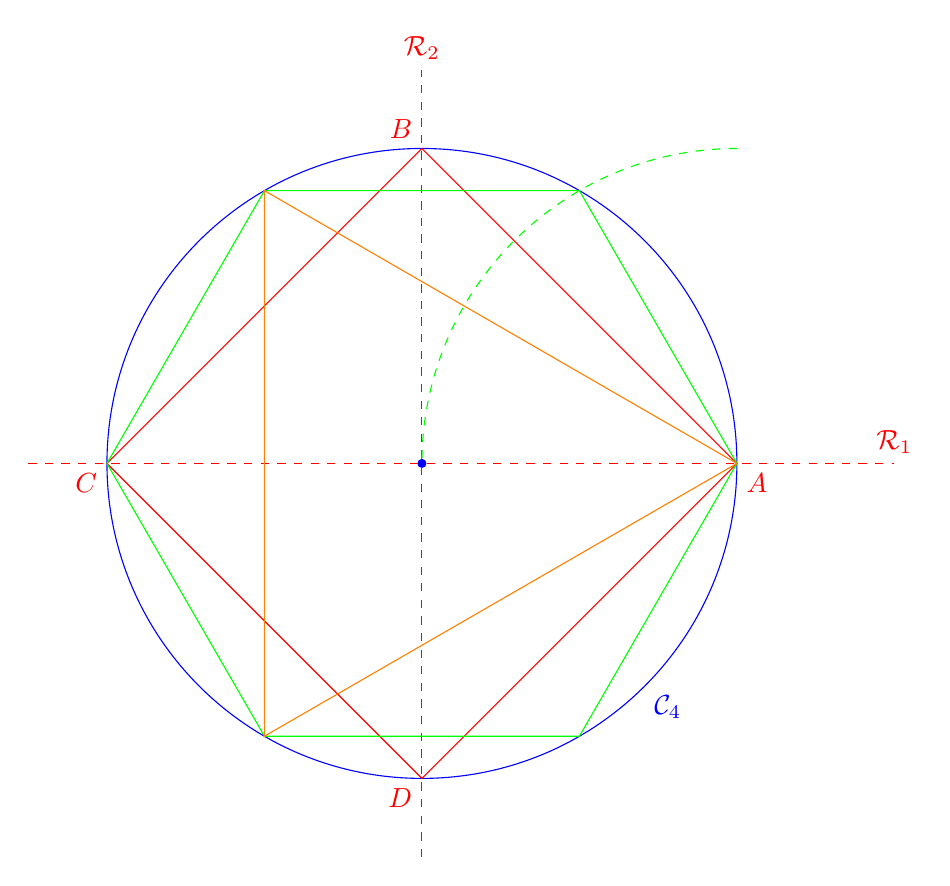
\begin{tikzpicture}
  \draw (0,0) circle(4)[color=blue];
  \draw[color=blue]
  (2.82842712474619,-2.82842712474619)node[below right]{$\mathcal{C}_4$};
  \draw[fill=black] (0,0) circle(.05)[color=blue];
  \draw (-5,0) -- (6,0)[dashed,color=red] node[above]{$\mathcal{R}_1$};
  \draw (0,-5) -- (0,5)[dashed,color=red] node[above]{$\mathcal{R}_2$};
  \draw[color=red] (4,0) node[below right]{$A$} -- (0,4) node[above left]{$B$}
  -- (-4,0) node[below left]{$C$} -- (0,-4) node[below left]{$D$} -- cycle;
  \draw (4,4) arc(90:180:4)[dashed,color=green];
  \draw (4,0) -- (2,3.464101615137754) -- (-2,3.464101615137754) --
  (-4,0) -- (-2,-3.464101615137754) -- (2,-3.464101615137754) -- (4,0)
        [color=green];
  \draw (4,0) -- (-2,3.464101615137754) -- (-2,-3.464101615137754) -- (4,0)
        [color=orange];
\end{tikzpicture}
\end{center}

On a separate figure,
we now draw $\mathcal{C}_3$ (orange)
and one of its diameter $\mathcal{D}$ (green).
We construct $E$ and $\mathcal{C}_1$ (cyan) and finally get three segments
(red, yellow, red).

\begin{center}
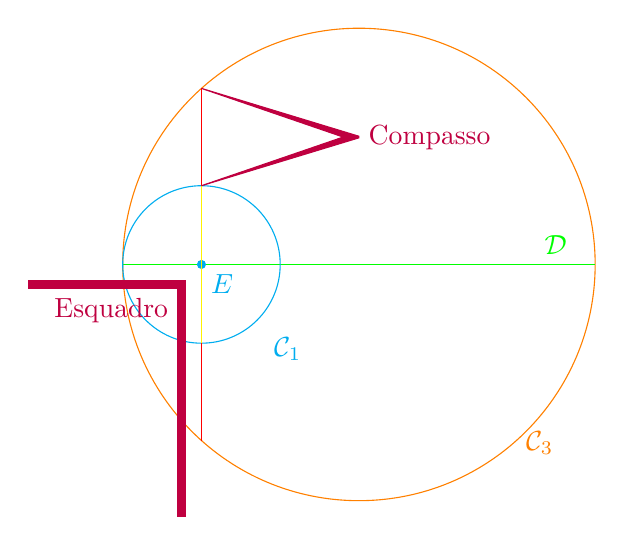
\begin{tikzpicture}
  \draw (0,0) circle(3)[color=orange];
  \draw[color=orange]
  (2,-2)node[below right]{$\mathcal{C}_3$};
  \draw[color=green](-3,0) -- (2.5,0)node[above]{$\mathcal{D}$} -- (3,0);
  \draw[fill=black] (-2,0) circle(.05)[color=cyan] node[below right] {$E$};
  \draw (-2,0) circle(1)[color=cyan];
  \draw[color=cyan]
  (-1.2,-.8)node[below right]{$\mathcal{C}_1$};
  \draw[color=red](-2,2.23606797749979) -- (-2,1);
  \draw[color=yellow](-2,1) -- (-2,-1);
  \draw[color=red](-2,-2.23606797749979) -- (-2,-1);

  \draw[color=purple,fill=purple](-2,2.23606797749979) --
  (0,1.628033988749895) -- (0,1.608033988749895) node[right]{Compasso} --
  (-2,1) -- (-.2,1.618033988749895) -- cycle;

  \begin{scope}[shift={(-.2,-.2)}]
  \draw[color=purple,fill=purple](-2,0) --
  (-4,0) -- (-4,-.1) -- (-2.1,-.1) node[below left]{Esquadro} --
  (-2.1,-3) -- (-2,-3) -- cycle;
  \end{scope}
\end{tikzpicture}
\end{center}

Using the compasso, we can report the length of a red segment to the original
figure and draw
$\mathcal{C}_{\sqrt{5}-1}$. We finally obtain a regular pentagon (green).

\begin{center}
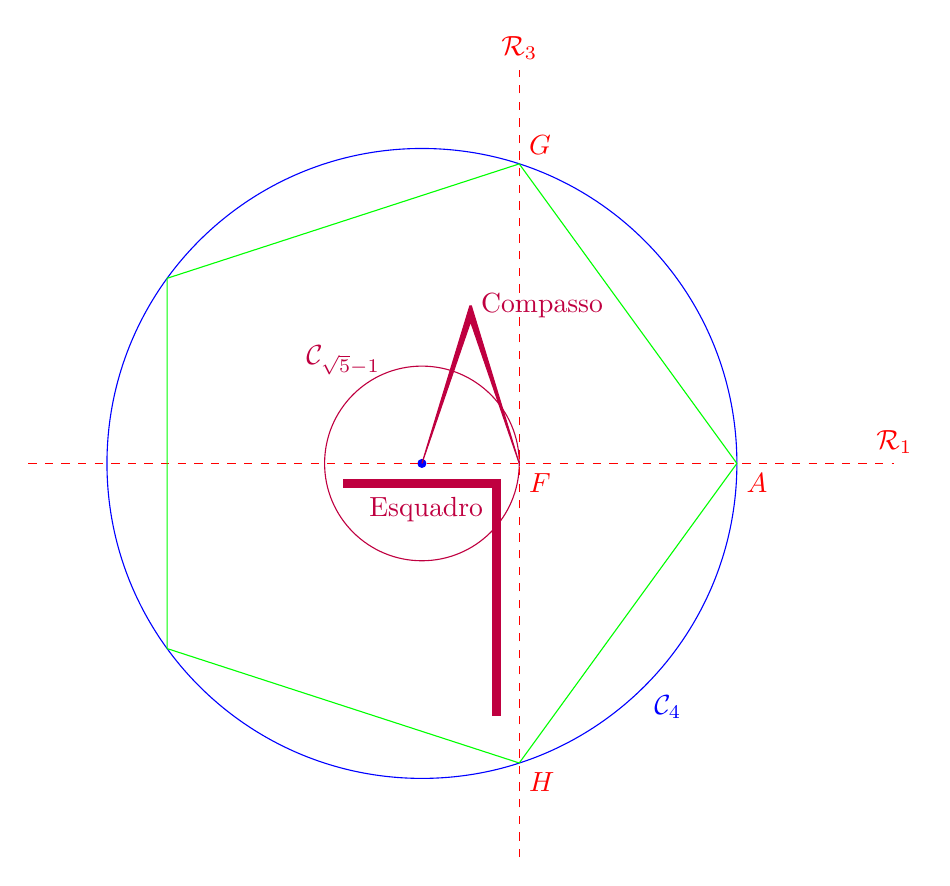
\begin{tikzpicture}
  \draw (0,0) circle(4)[color=blue];
  \draw[color=blue]
  (2.82842712474619,-2.82842712474619)node[below right]{$\mathcal{C}_4$};
  \draw[fill=black] (0,0) circle(.05)[color=blue];
  \draw (-5,0) -- (6,0)[dashed,color=red] node[above]{$\mathcal{R}_1$};
  \draw[color=red] (4,0) node[below right]{$A$};
  \draw (0,0) circle(1.236067977499789)[color=purple];
  \draw[color=purple](-1,1)node[above]{$\mathcal{C}_{\sqrt{5}-1}$};
  \draw (1.236067977499789,-5) -- (1.236067977499789,5)[dashed,color=red] node[above]{$\mathcal{R}_3$};
  \draw[color=red] (1.236067977499789,0) node[below right]{$F$};
  \draw[color=red] (1.236067977499789,3.804226065180614) node[above right]{$G$};
  \draw[color=red] (1.236067977499789,-3.804226065180614) node[below right]{$H$};
  \draw[color=green]
  (4, 0) --
  (1.23606797749979,3.804226065180614) --
  (-3.236067977499789,2.351141009169893) --
  (-3.236067977499789,-2.351141009169892) --
  (1.23606797749979,-3.804226065180614) -- 
  (4,0);

  \begin{scope}[rotate=90,shift={(2,-2.23606797749979)}]
  \draw[color=purple,fill=purple](-2,2.23606797749979) --
  (0,1.628033988749895) -- (0,1.608033988749895) node[right]{Compasso} --
  (-2,1) -- (-.2,1.618033988749895) -- cycle;
  \end{scope}

  \begin{scope}[shift={(3,-.2)}]
  \draw[color=purple,fill=purple](-2,0) --
  (-4,0) -- (-4,-.1) -- (-2.1,-.1) node[below left]{Esquadro} --
  (-2.1,-3) -- (-2,-3) -- cycle;
  \end{scope}

\end{tikzpicture}
\end{center}

Construyendo las bisecrices de los ángulos centrales del pentagono
obtenemos un decágono regular (naranja)
inscrito en $C$. De la misma manera, a partir del cuadrado y hexágono
obtenemos octógono y dodecágono regulares inscritos en $C$. Y a partir del
octógono, obtenemos un hexadecágono.

\begin{center}
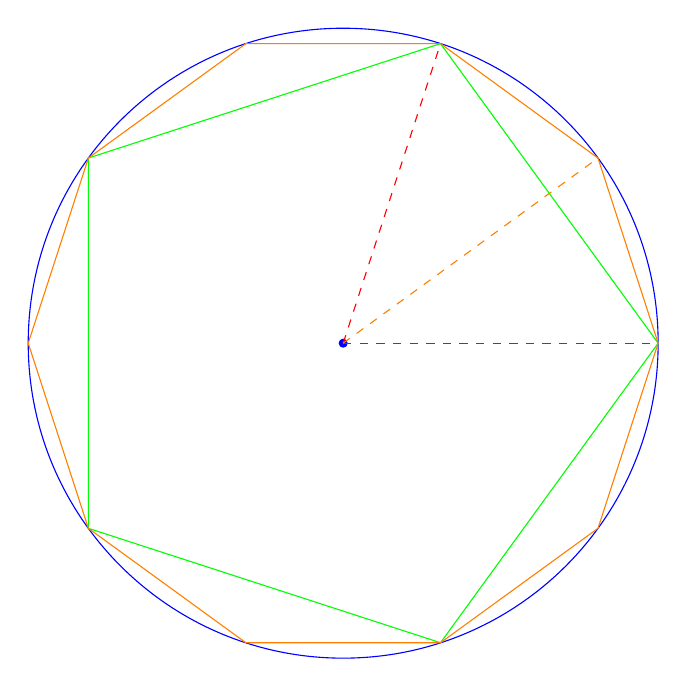
\begin{tikzpicture}
  \draw (0,0) circle(4)[color=blue];
  \draw[fill=black] (0,0) circle(.05)[color=blue];
  \draw[color=green]
  (1.23606797749979,3.804226065180614) --
  (-3.236067977499789,2.351141009169893) --
  (-3.23606797749979,-2.351141009169892) --
  (1.23606797749979,-3.804226065180614) -- (4, 0) --
  (1.23606797749979,3.804226065180614);
  \draw[dashed,color=red] (0,0) -- (4,0);
  \draw[dashed,color=red] (0,0) -- (1.23606797749979,3.804226065180614);
  \draw[dashed,color=orange] (0,0) -- (3.23606797749979,2.351141009169892);
  \draw[color=orange]
  (4,0) --
  (3.23606797749979,2.351141009169892) --
  (1.23606797749979,3.804226065180614) --
  (-1.23606797749979,3.804226065180614) --
  (-3.236067977499789,2.351141009169893) --
  (-4,0) --
  (-3.23606797749979,-2.351141009169892) --
  (-1.23606797749979,-3.804226065180614) --
  (1.23606797749979,-3.804226065180614) --
  (3.236067977499789,-2.351141009169893) --
  (4, 0);

\end{tikzpicture}
\end{center}

Utilizando las construciones del triángulo equilátero y del pentágono regular,
podemos construir el ángulo $2\alpha - \beta =
2 \times \frac{360}{5} - \frac{360}{3} = \frac{360}{15}$. Eso nos permite
construir un pentadecágono ($15$-gono) regular inscrito en $C$.

\begin{center}
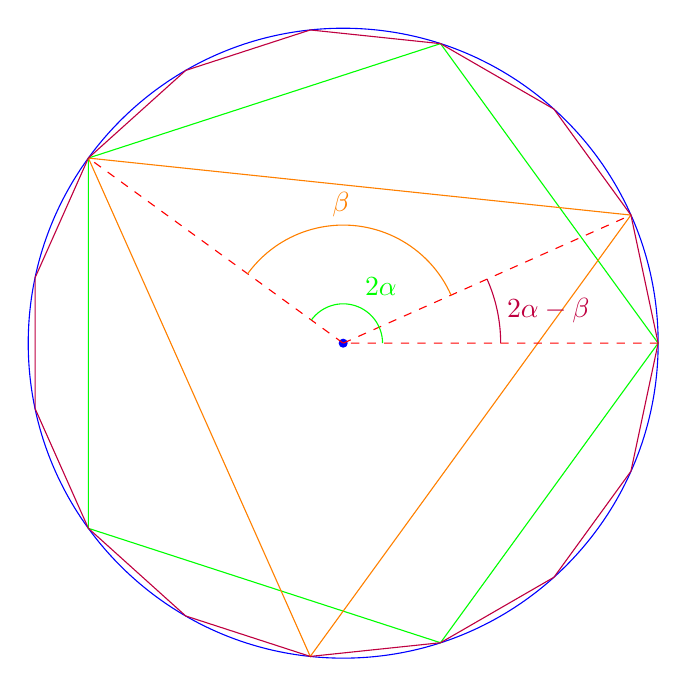
\begin{tikzpicture}
  \draw (0,0) circle(4)[color=blue];
  \draw[fill=black] (0,0) circle(.05)[color=blue];
  \draw[color=green]
  (4, 0) --
  (1.23606797749979,3.804226065180614) --
  (-3.236067977499789,2.351141009169893) --
  (-3.23606797749979,-2.351141009169892) --
  (1.23606797749979,-3.804226065180614) -- 
  (4,0);
  \draw[color=orange]
  (-3.236067977499789,2.351141009169893) -- (3.654181830570403,1.6269465723032)
  -- (-0.41811385307061,-3.978087581473093) --
  (-3.236067977499789,2.351141009169893);
  \draw[dashed,color=red]
  (4,0) -- (0,0) -- (-3.236067977499789,2.351141009169893);
  \draw[dashed,color=red]
  (0,0) -- (3.654181830570403,1.6269465723032);
  \draw[color=green] (.5,0) arc (0:72:.5) node[above right]{$2\alpha$} 
  arc (72:144:.5);
  \draw[color=orange] (1.370318186463901,0.6101049646137) arc (24:100:1.5)
  node[above right]{$\beta$} arc (100:144:1.5);

  \draw[color=purple] (2,0) arc (0:12:2)
  node[right]{$2\alpha-\beta$} arc (12:24:2);

  \draw[color=purple] (4,0) -- 
  (3.654181830570403,1.6269465723032)--
  (2.676522425435433,2.972579301909576) --
  (1.236067977499789,3.804226065180614) --
  (-0.41811385307061,3.978087581473093) --
  (-2.0,3.464101615137754) --
  (-3.236067977499789,2.351141009169893) --
  (-3.912590402935222,0.83164676327103) --
  (-3.912590402935222,-0.83164676327103) --
  (-3.236067977499789,-2.351141009169893) --
  (-2.0,-3.464101615137754) --
  (-0.41811385307061,-3.978087581473093) --
  (1.236067977499789,-3.804226065180614) --
  (2.676522425435433,-2.972579301909576) --
  (3.654181830570403,-1.6269465723032) --
  (4,0);
\end{tikzpicture}
\end{center}

We measure the following angles with a transferidor:

\begin{center}
\begin{tabular}{| c | c  | c |}
\hline
Number of sides $n$ & Central angle & Interior angle \\
\hline
$3$ & $120°$ & $60°$ \\
\hline
$4$ & $90°$ & $90°$ \\
\hline
$5$ & $72°$ & $108°$ \\
\hline
$6$ & $60°$ & $120°$ \\
\hline
$8$ & $45°$ & $135°$ \\
\hline
$10$ & $36°$ & $144°$ \\
\hline
$12$ & $30°$ & $150°$ \\
\hline
$15$ & $24°$ & $156°$ \\
\hline
$16$ & $22.5°$ & $157.5°$ \\
\hline
\end{tabular}
\end{center}

By Exercício 5, the sum of central angles is $360°$ while the sum
of interior angles is $180° \times {(n-2)}$. Because the $n$-gon is regular,
all central angles measure $\frac{360°}{n}$ and all interor angles
measure $180° \times \frac{n-2}{n}$.

Each regular polygon has a simetria de rotação of center the center of the
polygon and grau de simetria rotacional $n$. There are also $n$ axiales
de simetria. If $n$ is even then half of these axes pass through two opposite vertices, and the other half through the midpoint of opposite sides.
If $n$ is odd then all axes pass through a vertex and the midpoint of the
opposite side.

By Exercício 6, we didn't need the esquadro to draw orthogonal lines. Also
we don't really need an exact metrics in $\text{cm}$. Instead, we can choose
an arbitrary unit segment and report its size using the compasso.
As a consequence, this exercise shows how to construct regular $n$-gons
with only rule and compasso. One can prove that these are all
the constructible $n$-gons with rule and compasso for $n \leq 16$.
It is well-known that Gauss also gave a construction of the regular
heptadecagon ($n=17$ sides).

\subsection*{Exercício 9}

We have find $F=12$, this is a regular dodecaedro. We also find $A=30$ and
$V=20$. We have $F+V=32=A+2$.

\subsection*{Exercício 10}

\begin{enumerate}
\item For example 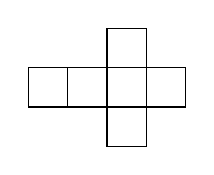
\begin{tikzpicture}
    \draw (0,0) -- (.5,0) -- (.5,.5) -- (0,.5) -- cycle
    (.5,0) -- (1,0) -- (1,.5) -- (.5,.5)
    (1,0) -- (1.5,0) -- (1.5,.5) -- (1,.5)
    (1.5,0) -- (2,0) -- (2,.5) -- (1.5,.5)
    (1,0) -- (1,-.5) -- (1.5,-.5) -- (1.5,0)
    (1,.5) -- (1,1) -- (1.5,1) -- (1.5,.5);
  \end{tikzpicture}

\item $V=8$, $A=12$, $F=6$ ; $F+V=14=A+2$.
\item

    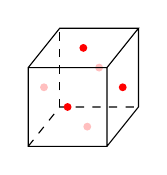
\begin{tikzpicture}
      \draw[dashed](0,0)--(.4,.5)--(1.4,.5);
      \draw[dashed](.4,.5)--(.4,1.5);
      \fill[pink] (.2,.75) circle(.05);
      \fill[pink] (.75,.25) circle(.05);
      \fill[pink] (.9,1) circle(.05);
      \fill[red] (.5,.5) circle(.05);
      \fill[red] (.7,1.25) circle(.05);
      \fill[red] (1.2,.75) circle(.05);
      \draw(0,0) -- (1,0) -- (1,1) -- (0,1) -- cycle
           (0,1) -- (.4,1.5) -- (1.4,1.5) -- (1,1)
           (1,0) -- (1.4,.5) -- (1.4,1.5);
    \end{tikzpicture}


\item This is a regular octaedro, with faces that are equilateral triangles.
  We have $V=6$, $A=12$ and $F=8$ so again $F+V=14=A+2$.
\end{enumerate}
